\begin{tframe}{Ontology Selection}
The \gls{eurio}: data model that formalizes and makes available structured, machine-readable data on EU-funded research projects.

\begin{columns}
    \begin{column}{0.48\textwidth}
      \vspace{-.5cm}
        \begin{itemize}
            \item Semantic model of research information, e.g., projects, calls, funding schemes, organizations, people \ldots
            \vspace{.2cm}
            \item \textbf{\gls{eurio} \gls{kg}} \cite{CORDIS_EURIO_2022}: an \acrshort{rdf} \gls{kg} built from \gls{cordis} data
        \end{itemize}
    \end{column}
    \begin{column}{0.48\textwidth}
      \begin{figure}
        \centering
        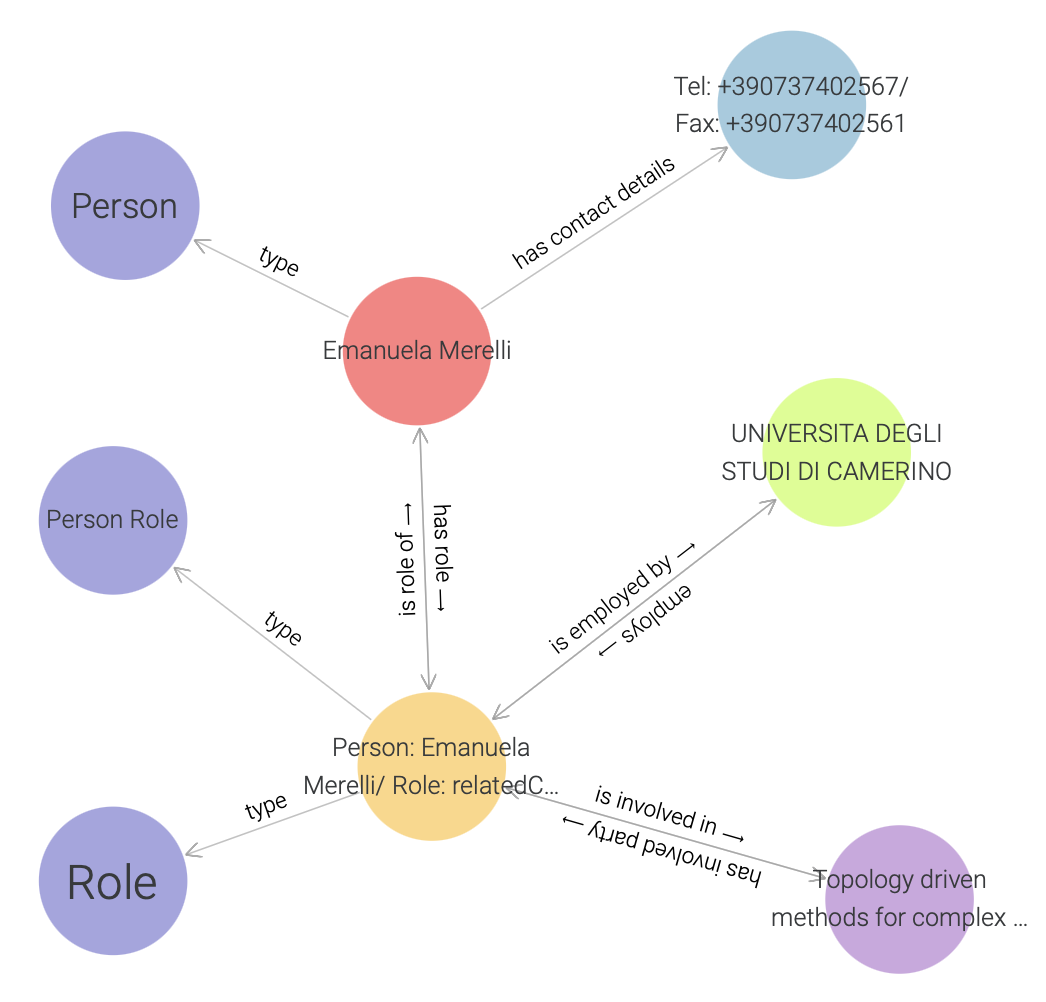
\includegraphics[width=.95\linewidth]{../img/architecture/example-merelli.png}
      \end{figure}
    \end{column}
  \end{columns}

\end{tframe}